\section{Methodology}

The open dataset for this study involves the collection of 227 gravity stations (Figure~\ref{geology}b). The Gravity measurements were obtained using a Lacoste and Romberg gravimeter (model G, ±0.01 mGal), while orthometric altitude was determined using a Differential Global Positioning System (DGPS) device (± 0.3 m). Data on gravity were collected at varying intervals: 

\begin{enumerate}[label=(\roman*)]
    \item detailed: with one station approximately every 0.3 km, forming three profiles intersecting the SAIC (Figure~\ref{geology}b), two traversing each lobe, and one along the internal shear zone.
    \item regional: in the country rocks, the data coverage was approximately one station per 4 km, aiming to complement the existing regional gravity dataset.
\end{enumerate}


The Bouguer anomaly was obtained and interpreted by \citet{Souza-Junior2021}. However, in this study, we will calculate the gravity field at the same point on the reference ellipsoid, thus obtaining the Bouguer disturbance. To accomplish this, a few processing stages were necessary, as it is described below.

\subsection{Altitude Transformation}\label{altitude}

The initial step involved converting orthometric altitudes ($H$) from both the gravimetric dataset in this study and the topographic database (with a spatial resolution of 30 m $\times$ 30 m, Figure~\ref{heights}a). To achieve this, we obtained the mesh containing the geoid level ($N$) for the study area (with an approximated spatial resolution of 10 km $\times$ 10 km, Figure~\ref{heights}b). The orthometric topography and geoid height databases were acquired from pyGMT database \citep{gmt} and plotted with the aid of the PyGMT library \citep{pygmt}. The geoid height grid underwent an interpolation process to generate a mesh with the same resolution as the orthometric topography, which was possible using the Verde python library \citep{verde2018}. Subsequently, the geometric altitude ($h$) was calculated by adding both meshes ($h = H + N$,~Figure~\ref{heights}c).

\begin{figure}[H]
  \centering
  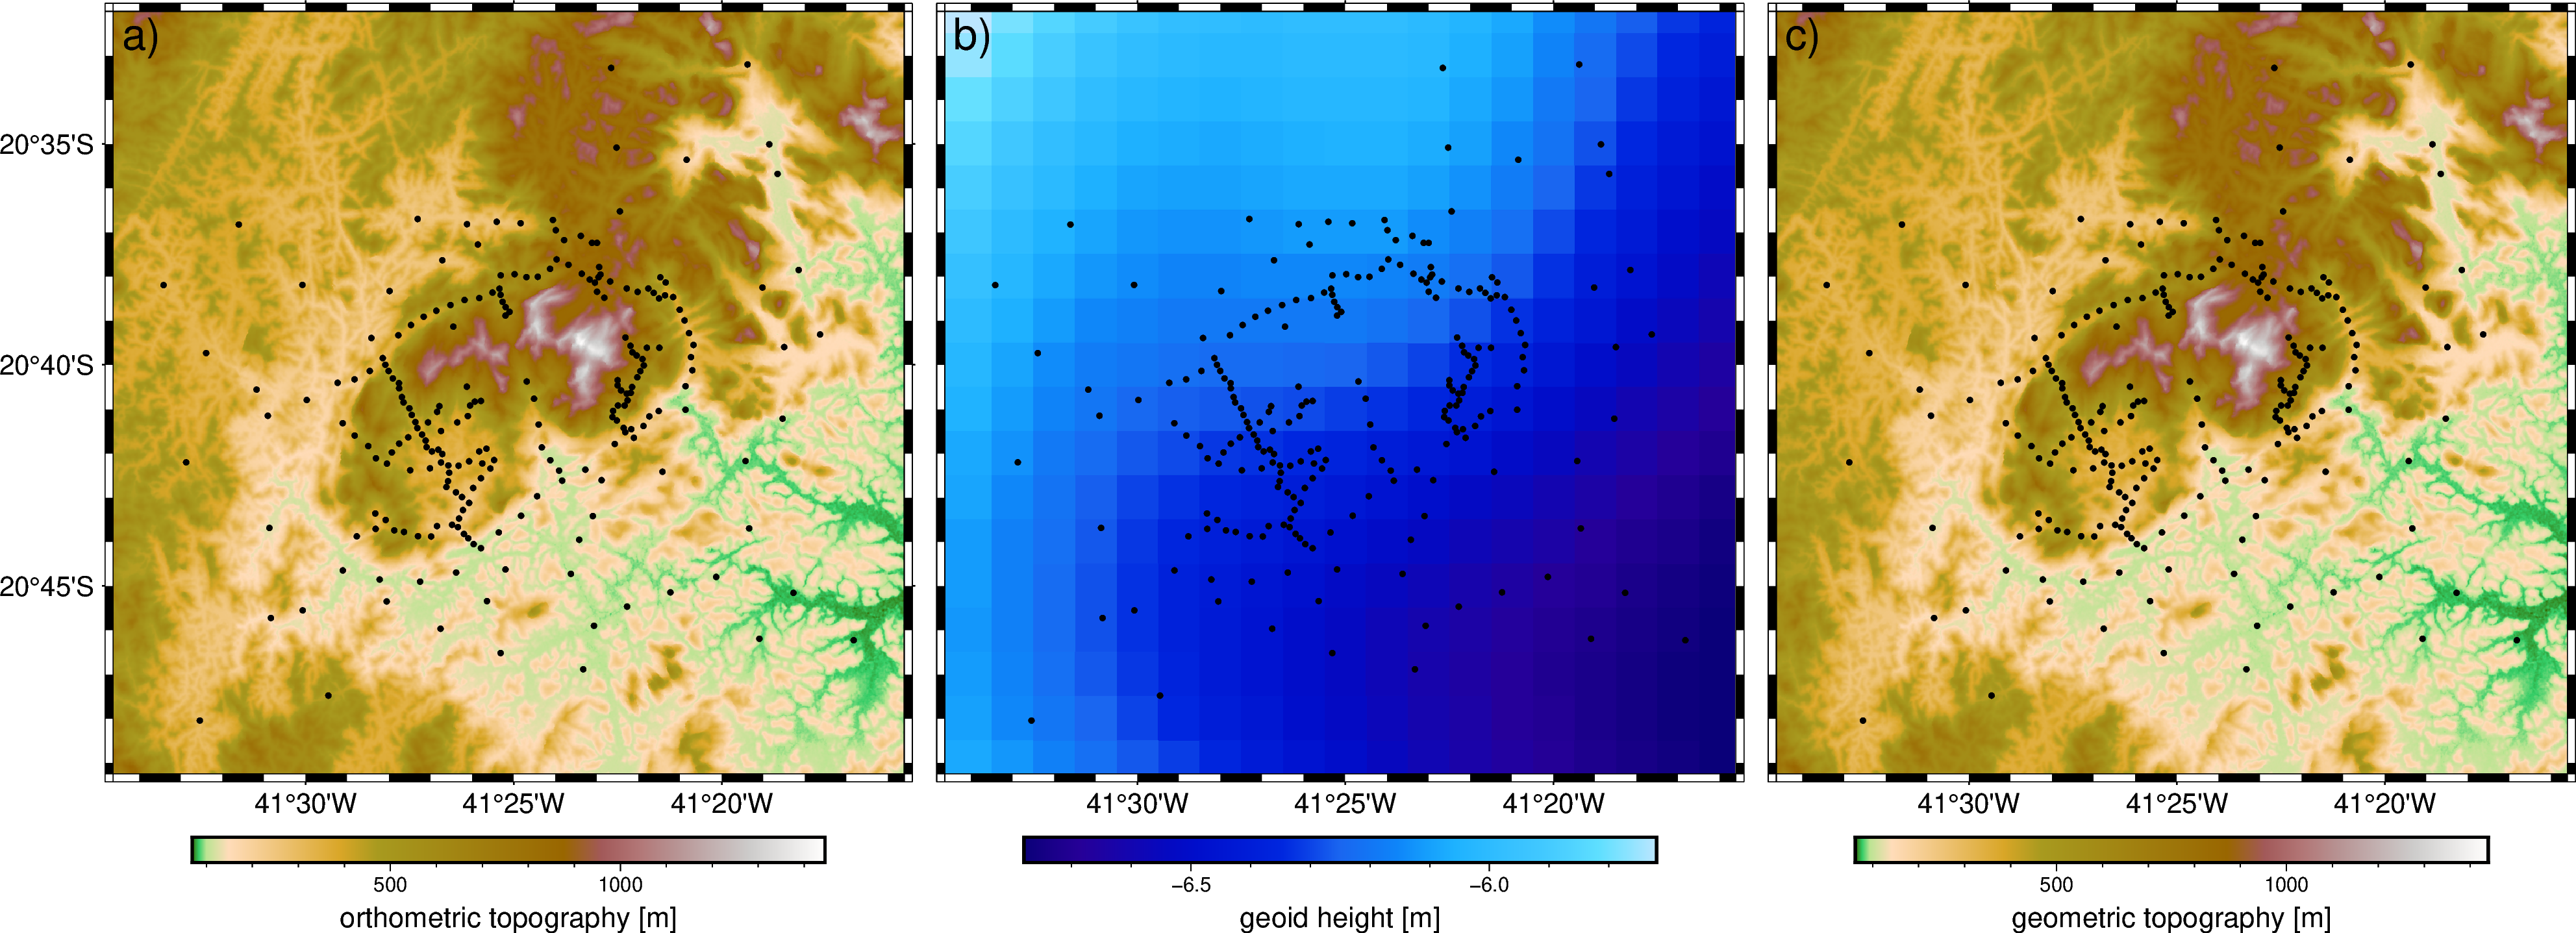
\includegraphics[width=1\linewidth]{figures/heights.png}
  \caption{
    Topographic grids of the study area. a) Orthometric topography. b) Geoid height. c) Geometric topography. 
      }
  \label{heights}
\end{figure}


\subsection{Normal Gravity}
An anomaly is usually a term related to the difference between a measured data (\textit{e.g.}, $g_{\text{obs}}$) and the theoretical or expected data in that specific point \citep{Encyclopedia_solid_earth_geophysics}. The calculation of the theoretical gravity is obtained with a model of a rotational bi-axial ellipsoid \citep{Pasteka2017}. This called ``normal Earth'' has a few characteristics: 

\begin{enumerate}[label=(\roman*)]
    \item The same mass (M) and center of mass as the Earth;
    \item The same angular velocity as the Earth; and
    \item The potential on its surface is equal to the potential of the geoid.
\end{enumerate}
The magnitude of the gradient of the gravity potential generated by the normal Earth ellipsoid, which includes the gravitational and centrifugal effects, is called normal gravity $(\gamma)$. The calculation of this normal gravity was performed using the World Geodetic System 1984 (WGS 84) by the Boule package \citep{Boule2020}, which implements the closed-form formula of \citet{Li2001} and calculate the $\gamma$ given the latitudes and the geometric heights. This is the reason why the first step consists of the conversion of the orthometric to geometric heights. 

\subsection{Topographic Correction}

Once the normal gravity is ``corrected'', a further correction must be performed to remove the effects of the rocks between the ellipsoid and the observation point, since the effect of the topography is not predicted in the theoretical gravity \citep{Encyclopedia_solid_earth_geophysics}. This called ``Bouguer correction'' ($\delta g_{B}$) usually is computed by an infinite slab of rock that fills the space between the geoid level and the measured point \citep{Lowrie1997}, \textit{i.e.}, the slab has the orthometric height ($H$). The Bouguer correction formula is given by:

\begin{equation}
{
\delta g_{B} = 2 \pi G \rho H},
\end{equation}

\noindent{where $G$ is the universal gravitational constant ($6.67428\times10^{-11}~m^3 kg^{-1} s^{-2}$) and and $\rho$ is the density of the Bouguer infinite-slab, which, by standard, generally assumes the crust's average density of $2670~kg~ m^{-3}$ \citep{Hinze2003}.}

However, this presumption of an infinite-slab can lead to errors in areas with very pronounced topographic variations and/or when the choice of plate density is made incorrectly \citep{Chapin1996}. Figure~\ref{heights} shows that the study area has topographic variations greater than 1000 meters, which will most likely cause unwanted calculation errors. Thus, it is possible to apply a method of topographic correction \citep[\textit{e.g.,}][]{Nagy2000} based on the topography mesh (Section~\ref{altitude}), since our goal is to determine the gravity disturbance we will use the geometric heights. In this sense, each grid cell of the digital elevation model was converted into a flat prism of 30 m $\times$ 30 m $\times$ $h$ m, this creates a volumetric model for the geometric topography. Subsequently, the gravity effect of each regular prism with a constant density ($\rho = 2670~kg~m^{-3}$) can be computed, which gives the topography's gravity effect ($g_T$).

\subsection{Bouguer Disturbance}
Depending on the chosen reference gravity model, two distinct types of anomaly variations might be considered: gravity anomalies and gravity disturbances. The geodetic gravity anomaly is defined as the distinction between gravity on the geoid and normal gravity on the reference ellipsoid \citep{Blakely1996}. Conversely, the gravity disturbance is defined as the difference in the fields at the same point on the reference ellipsoid. According to \citet{Encyclopedia_solid_earth_geophysics} the gravity disturbances are more suitable for geophysical purposes. When applying the normal gravity and terrain corrections, the Bouguer disturbance ($\delta g_{b}$) can be determined by:

\begin{equation}
{
\delta g_{b} = g_{obs} - \gamma - g_T}.
\end{equation}

\subsection{Residual-Regional Separation}

The Bouguer anomaly, or Bouguer disturbance in this case (Figure~\ref{gravity}a), is said to be the result from the density contrast between rocks \citep{Amelio1997}. However, potential fields are additives and usually consist of two components: one with large-wavelength and other with short-wavelength. Anomalies of large wavelength are caused by the effects of deeper density contrasts and are referred to as regional anomalies \citep{Telford1990}. On the other hand, short-wavelength anomalies, known as residual anomalies, are induced by anomalous mass distribution in the shallow crust and are employed for their study \citep{Lowrie1997}. Therefore, studying more restricted area requires the application of a regional-residual separation technique to isolate the effect of the targeted bodies. 

In our study, we applied a first-degree polynomial fit onto the Bouguer disturbance map (Figure~\ref{gravity}a) to predict the regional component of the regional/deeper sources using Verde python package \citep{verde2018}, as shown in Figure~\ref{gravity}b. Then, this regional trend was subtracted from the Bouguer disturbance to generate the residual anomalies map (Figure~\ref{gravity}c).
These anomalies, or residuals, are attributed to localized and shallow subsurface bodies.

\begin{figure}[H]
  \centering
  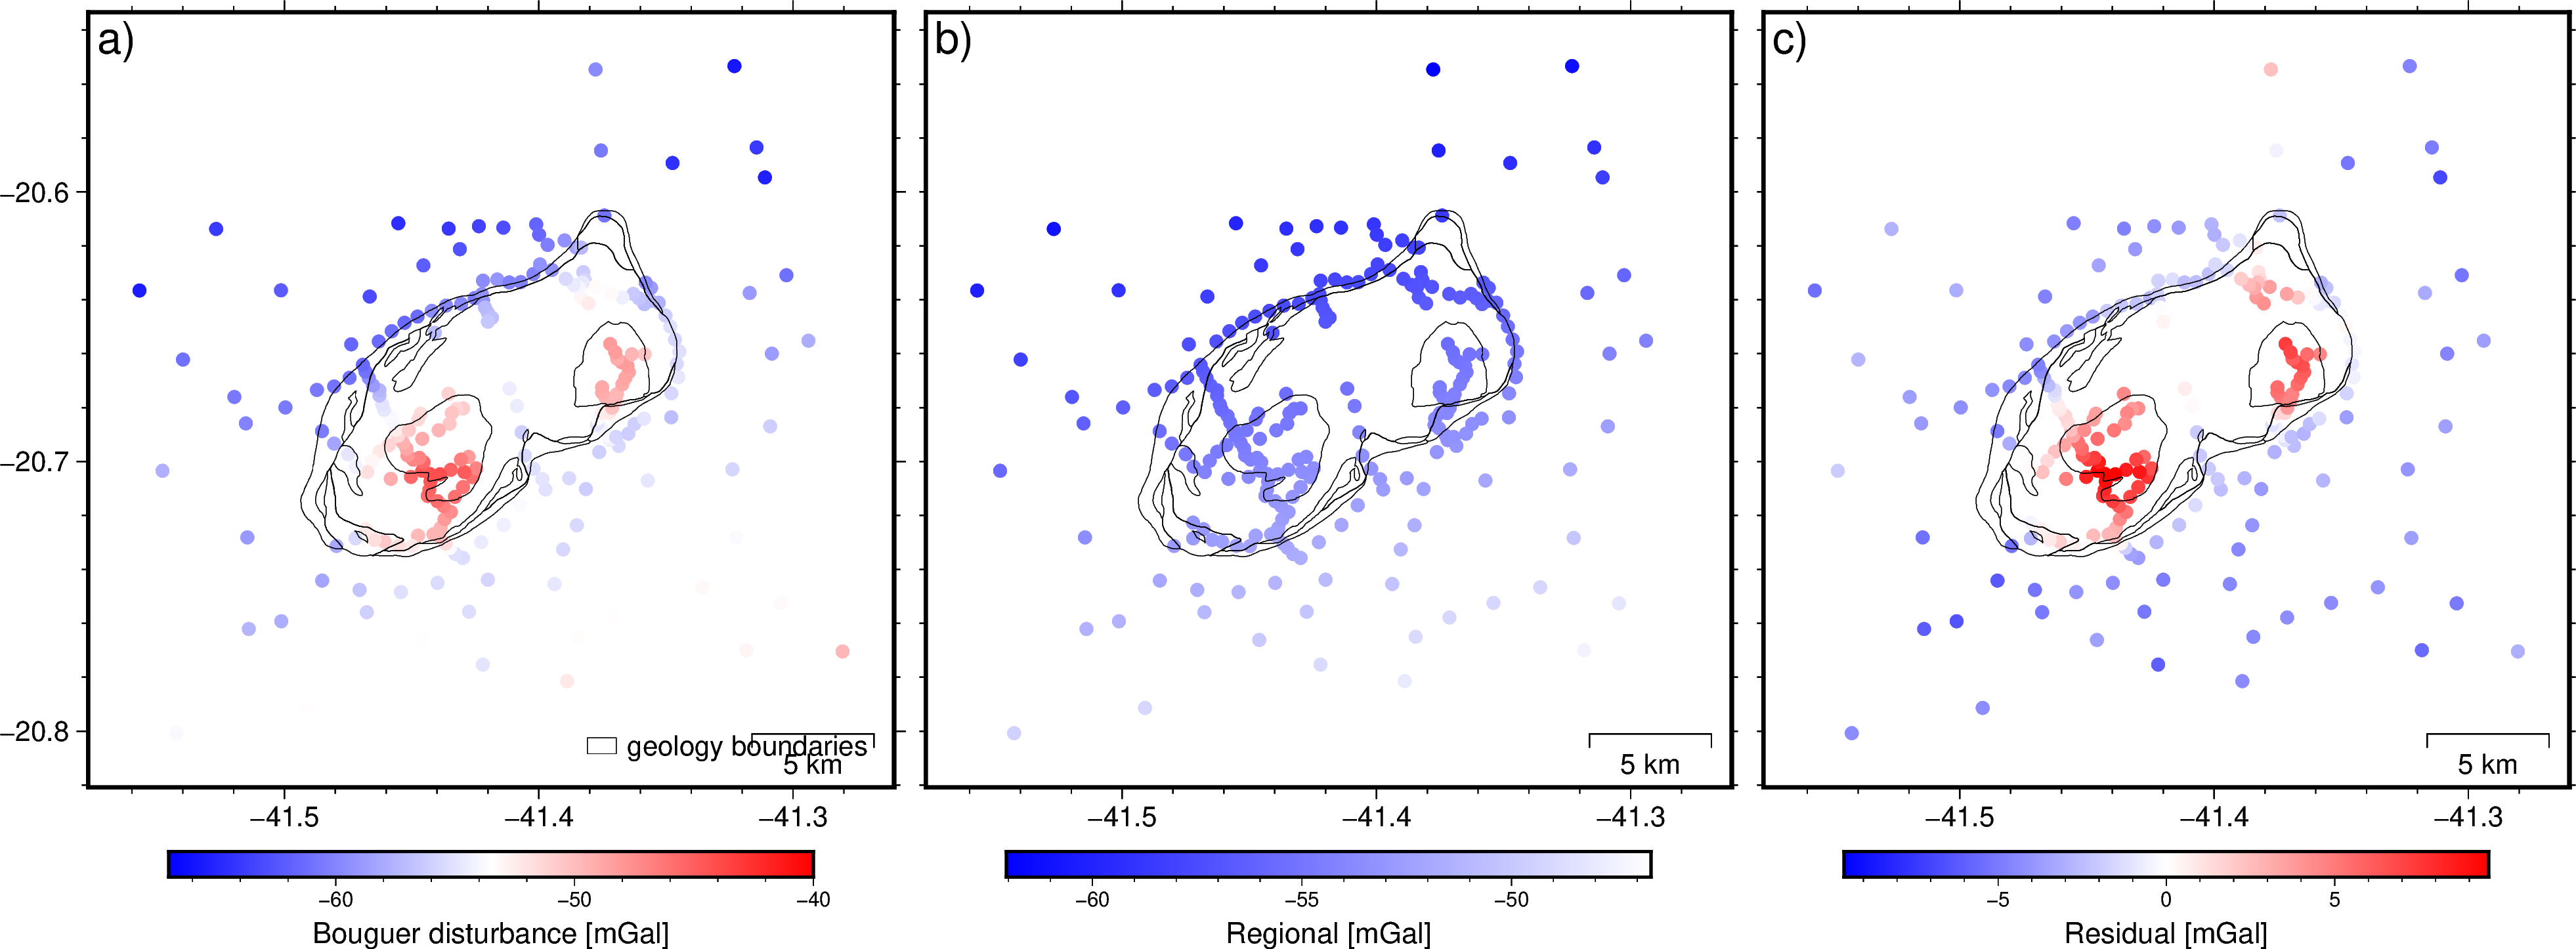
\includegraphics[width=1\linewidth]{figures/gravity.png}
  \caption{
    SAIC's gravimetric maps. a) Bouguer disturbance. b) Regional anomaly obtained with the first-degree polynomial fit of the Bouguer disturbance. c) Residual Bouguer disturbance.
      }
  \label{gravity}
\end{figure}


\subsection{Data Interpolation with Equivalent Layer}

Potential field surveys often are datasets of irregular measurements from flight lines or along the terrain's surface. The processing usually involves interpolating onto a regular grid at a constant height for further visualization and processing (\textit{e.g.,} reduction-to-the-pole, upward continuation and derivatives calculations) \citep{Soler2021}. An effective method for performing this task is through equivalent sources \citep{Dampney1969}, also known as an equivalent layer. This technique involves defining a finite set of geometric bodies (e.g., point sources) beneath observation points and adjusting their coefficients to replicate the measured field. The technique can be used to predict the values for the gravimetric and magnetic field at any point, such as regular grids and different heights, while also outperforming others 2D interpolators like the minimum curvature or bi-harmonic splines \citep{Soler2020, Uieda2020}.

\subsubsection{Derivatives and Gradients}

With the same equivalent layer it is possible do determine derivatives by disturbing the regular grid with a value $\Delta \alpha$, $\alpha = x, y, z$, and predicting the residual Bouguer disturbance at that point, following the finite-difference method:

\begin{equation}
    {\frac{\partial f}{\partial x} = \frac{f(x + \Delta x, y, z) - f(x - \Delta x, y, z)}{2\Delta x}},
\end{equation}

\noindent{likewise for the other derivatives. Afterwards, they can be applied on the formulas:

\begin{align}
    HG &= \sqrt{\left (\frac{\partial f}{\partial x}\right )^2+\left (\frac{\partial f}{\partial y} \right )^2}~~~~~~~~~\text{and} \\
    TG &= \sqrt{\left (\frac{\partial f}{\partial x}\right )^2+\left (\frac{\partial f}{\partial y} \right )^2+\left (\frac{\partial f}{\partial z} \right )^2},
\end{align}

\noindent{so it is possible to calculate the horizontal gradient \citep[HG,][]{Cordell1985} and the total gradient \citep[TG,][]{Roest1992Magnetic}.}
